\section{\emph{OOC - \emph{Object Orientated Programming in ANSI-C}}}
Segundo \cite{schreiner1993object}, OOC, \emph{Object Orientated Programming in ANSI-C}, é uma forma de se aproveitar as diversas vantagens da Programação orientada objeto. Vantagens essas proporcionadas por linguagens como C++, java, python, smalltalk e outras. OOC, necessita da separação em dois arquivo distintos, semelhante a do c++: o primeiro possui a extensão por padrão ".h" e contém apenas a declarações de interfaces e classes, já o segundo, com extensão ".c", possui a devida implementação. Este é um conceito considerado mais denso do que Orientação Objeto propriamente dito, isso se deve ao fato de que o usuário implemente componentes como: 

\begin{itemize}
\item Interface: Define-se interface como uma \emph{struct} com ponteiros para funções, de forma que o \emph{bind} das funções é feito na hora da criação de um objeto de uma classe que implemente essa interface;
\item Classe: Da mesma forma que as interfaces, é uma \emph{struct} em que os atributos são ponteiros para função, entretanto tem os \emph{binds} definidos em uma função de criação(construtor) pertencente a essa classe, ou módulo;
\item Construtor: Função da classe em que faz o \emph{bind} de cada ponteiro para cada função da classe, alocações dinâmicas e outras operações que podem ser definidas de acordo com a necessidade de cada classe;
\item Destrutor: Basicamente a liberação de todos os recursos alocados pelo construtor e funções que a classe utilizou;
\item Public: Declaração da variável como atributo da \emph{struct} ou no arquivo \emph{header};
\item Private: Declaração da variável fora da \emph{struct}, no arquivo que tem a implementação das funções da classe.
\end{itemize}

O conceito de polimorfismo e abstração de dados se dá pela associação de um mesmo ponteiros de função de uma classe ou interface à funções diferente, variando em função da classe mais especializada que está sendo abstraída.

Obviamente é uma simulação da consolidada programação orientada objeto e possui limitações como: Programação genérica sem validação em tempo de compilação, sintaxe mais complexa, geração de código implícito, entre outros. Entretanto ainda permite reutilização de código e, como dito anteriormente, abstração de dados.

\section{\emph{Design Patterns}}
Na engenharia de \emph{software}, um \emph{Design Patterns} ou padrão de projeto é uma solução repetível geral para um problema comumente ocorre em \emph{design} de \emph{software}. Um padrão de projeto não é um projeto acabado que pode ser transformado diretamente em código. É uma descrição ou modelo de como resolver um problema que pode ser utilizado em diversas situações diferentes. \cite{shalloway2004design}.

\subsection{Usos de \emph{Design Patterns}}

Os \emph{Design Patterns} podem acelerar o processo de desenvolvimento, fornecendo testados e comprovados paradigmas de desenvolvimento. O \emph{design} de \emph{software} eficaz requer considerar as questões que não podem tornar-se visível até mais tarde na implementação. Reutilizar \emph{Design Patterns} ajuda a prevenir situações que podem causar grandes problemas e melhora a legibilidade do código para programadores e arquitetos familiarizados com os padrões.

Muitas vezes, as pessoas só entendem como aplicar certas técnicas de \emph{design} de \emph{software} para determinados problemas. Estas técnicas são difíceis de aplicar a uma ampla gama de problemas. Os \emph{Design Patterns} fornecem soluções gerais, documentadas em um formato que não requer especificidades ligadas a um problema particular \cite{shalloway2004design}.

Segundo \cite{shalloway2004design}, além disso, os padrões permitem que os desenvolvedores se comuniquem usando nomes bem conhecidos e bem compreendidos para interações de software. \emph{Design Patterns} comuns podem ser melhorados ao longo do tempo, tornando-os mais robustos do que os projetos ad-hoc, ou seja, problemas específicos. Os \emph{Design Patterns} podem ser divididos em:

\begin{itemize}
\item \emph{Creational design patterns}: Estes \emph{Design Patterns} tem tudo a ver com padrões de instanciação de classe. Esse padrão pode ser dividido em padrões de criação de classe e de criação de objetos. Enquanto os padrões de criação de classe usam a herança de forma eficaz no processo de instanciação, os padrões de criação de objeto usam a delegação de forma eficaz para ter o trabalho de criação feito. 
\item \emph{Structural design patterns}: Este \emph{Design Pattern} tem tudo a ver com composição de classe e objetos. Padrão estrutural de classe usa a herança para compor interfaces. Padrão estrutural de objeto define formas de compor objetos para obter novas funcionalidades.
\item \emph{Behavioral design patterns}: São os padrões que são mais especificamente relacionadas com a comunicação entre objetos.
\end{itemize}

\subsection{\emph{Factory Method}}
Segundo \cite{shalloway2004design}, \emph{factory method} foi um dos \emph{Design Patterns} escolhidos para esse projeto. Seus objetivos principais são:

\begin{itemize}
\item Definir uma interface para criar um objeto, mas deixa as subclasses decidirem qual classe instanciar. Factory Method permite adiar a instanciação da classe para a subclasses;
\item Definir um construtor \emph{virtual};
\item Operador \emph{new} é considerado perigoso.
\end{itemize}

Esse \emph{Design Patterns} foi utilizado no módulo que faz uso do \emph{display} de LCD para que a troca de seu tipo ficasse isolado do restante do sistema e que um futura troca possa ser feita com o menor impacto possível. A Figura \ref{fig:factorymethod} representa sua etsrutura em UML. \newpage

\begin{figure}[htp]
	\centering
	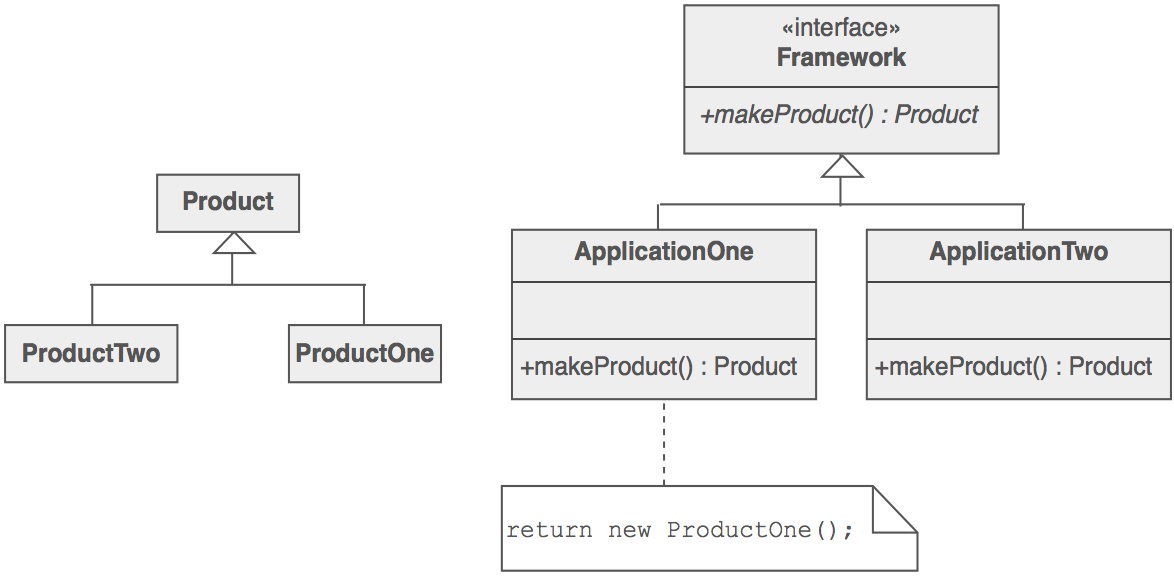
\includegraphics[scale=0.4]{images/Factory_Method.png}
	\caption{Estrutura do padrão \emph{Factory Method}}	
	\label{fig:factorymethod}
	\cite{shalloway2004design}
\end{figure}
